\documentclass[aspectratio=169,11pt,hyperref={colorlinks=true}]{beamer}
\usepackage[utf8]{inputenc}
\usepackage[T1]{fontenc}
\usepackage{fontspec}
\usepackage[absolute,overlay]{textpos}
\usepackage{listingsutf8}
\usepackage{listings-golang}
\usepackage{tikz}
\usepackage{color}
\usepackage{fontawesome5}
\usepackage{svg}


\title{From Zero to CD with Tekton}
\date[14 Apr 2021]{14 Apr 2021 | \faTwitter ~@blackchip76 | \faGithub ~afrittoli}
\author[Andrea Frittoli]{%
  Andrea Frittoli \\
  Developer Advocate \\
  andrea.frittoli@uk.ibm.com \\
}

\usetheme{af}

% Code style
\setlststyle

\lstdefinelanguage{koyaml}{
  keywords={github, com, afrittoli, examples, ms, go, helloworld},
  sensitive=false,
  comment=[l]{\#},
  morestring=[b]',
  morestring=[b]"
}

% Automatic section frame
% \AtBeginSection{\frame{\sectionpage}}

\begin{document}

\begin{frame}
\titlepage{}
\end{frame}

\begin{lpicrblack}[chewy-I-rgDPLKogs-unsplash.jpg]{%
  Photo by \href{https://unsplash.com/@chewy}{\underline{Chewy}}, CC0
  }%
  {%
  \tableofcontents
  }%
  {toc}
  \frametitle{Agenda}
\end{lpicrblack}

\section[Introduction]{Introduction}

\begin{sectionwithpic}[mike-benna-X-NAMq6uP3Q-unsplash.jpg]{Photo by \href{https://unsplash.com/@mbenna}{\underline{Mike Benna}}, CC0}
\end{sectionwithpic}

\begin{stripedframe}%
  {%
  Tekton is an open-source framework \\ for creating CI/CD systems \\ ~
  }%
  {%
  Cloud Native \\
  \vspace{0.03\textheight}
  Serveless, Scalable Pipelines \\
  \vspace{0.1\textheight}
  \centering
  \includesvg[width=0.08\paperwidth]{img/tekton-icon-white.svg}
  }%
  {%
  Standardization \\
  \vspace{0.03\textheight}
  Built In Best Practices \\
  \vspace{0.03\textheight}
  Maximum Flexibility \\
  }%
  {%
  Core Projects
  \begin{itemize}
    \item Pipeline
    \item Triggers
  \end{itemize}
  \vspace{0.01\textheight}
  Tooling:
  \begin{itemize}
    \item CLI \textit{tkn}
    \item Dashboard
    \item Operator
  \end{itemize}
  }%
  {%
  Discovery:
  \begin{itemize}
    \item Catalog
    \item Hub
  \end{itemize}
  \vspace{0.01\textheight}
  Adds-on:
  \begin{itemize}
    \item Results
    \item Chain
    \item Experiments
  \end{itemize}
  }%
  % \begin{textblock*}{0.13\paperwidth}(0.73\paperwidth,0.65\paperheight)
  %   \includesvg[width=0.13\paperwidth]{img/tekton-icon-color.svg}
  % \end{textblock*}
  % A brief into to Tekton
\end{stripedframe}

\begin{lgrayrwhiteframe}
  \frametitle{A bit of history}
  \begin{itemize}
    \item From Knative Built, to Pipeline
    \item Extend the k8s API with CRDs
    \item Tekton and the CDF
  \end{itemize}
  \vspace{0.03\paperheight}
  ~~~~~\includesvg[width=0.1\paperwidth]{img/cdf-stacked-color.svg}
  \vspace{0.03\paperheight}
  \begin{itemize}
    \item Definitions: Step, Task, Pipeline
    \item Bindings: Workspaces, Parameters, \\Results
    \item Execution: TaskRun, PipelineRun
  \end{itemize}
  \begin{textblock*}{0.51\paperwidth}(0.48\paperwidth,0.33\paperheight)
    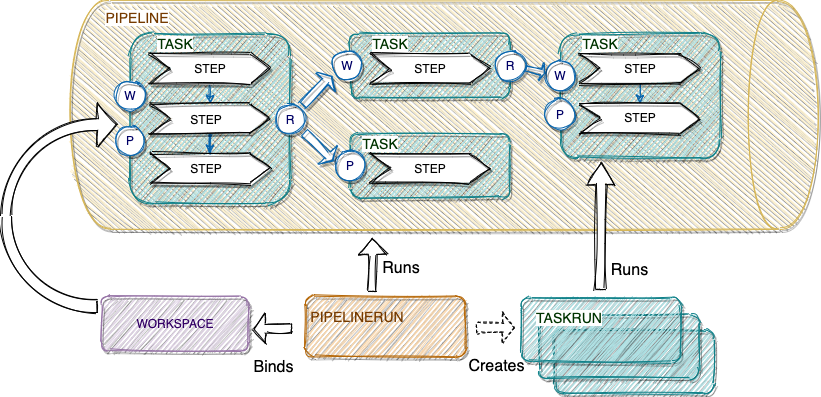
\includegraphics[width=0.5\paperwidth]{img/tekton-workspaces.png}
  \end{textblock*}
  % Knative, Tekton and the CDF
\end{lgrayrwhiteframe}

\section[From 0 to CD]{From 0 to CD}
\begin{sectionwithpicrx}[pierre-bamin--ltjzTfhpCI-unsplash.jpg]{Photo by \href{https://unsplash.com/@bamin}{\underline{Pierre Bamin}}, CC0}
\end{sectionwithpicrx}

\begin{blackframe}
  \frametitle{Install}
  \begin{itemize}
    \item Install
    \item Operator
    \item Nightly
    \item Multi-arch
  \end{itemize}
\end{blackframe}

\begin{blackframe}
  \frametitle{Authoring}
  \begin{itemize}
    \item pipeline
    \item catalog
    \item hub
    \item params, results, workspaces <- docs on website
  \end{itemize}
\end{blackframe}

\begin{blackframe}
  \frametitle{Watching}
  \begin{itemize}
    \item kubectl
    \item tkn
    \item Dashboard
    \item runtime aspects
  \end{itemize}
\end{blackframe}

\begin{blackframe}
  \frametitle{Launching}
  \begin{itemize}
    \item triggers
    \item setup a github webhook
    \item run a build on push
    \item filtering: CEL, custom, when expressions
  \end{itemize}
\end{blackframe}

\begin{blackframe}
  \frametitle{Monitoring}
  \begin{itemize}
    \item unattended execution, we need monitoring
    \item event
    \item cloudevents
    \item notifications (github, slack)
  \end{itemize}
\end{blackframe}

\begin{blackframe}
  \frametitle{Experimental}
  \begin{itemize}
    \item loops
    \item wait
    \item CELRun / pip (?)
  \end{itemize}
\end{blackframe}

\begin{blackframe}
  \frametitle{Cleanup}
  \begin{itemize}
    \item execution history
    \item results
  \end{itemize}
\end{blackframe}

\section[Roadmap]{Roadmap}
\begin{sectionwithpic}[pexels-ray-bilcliff-1509237.jpg]{Photo by \href{https://www.pexels.com/@raybilcliff}{\underline{Ray Bilcliff}}, CC0}
\end{sectionwithpic}

\begin{blackframe}
  \frametitle{TEP (optional)}
  \begin{itemize}
    \item Design principles
    \item TEP process
    \item TEP table
  \end{itemize}
\end{blackframe}

\begin{blackframe}
  \frametitle{Dogfooding (optional)}
  \begin{itemize}
    \item Using Tekton for Tekton
    \item Source of examples
    \item Source of bug discovery, feature requests
  \end{itemize}
\end{blackframe}

\begin{blackframe}
  \frametitle{Roadmap}
  \begin{itemize}
    \item Towards v1
    \item What's coming in 2021
    \item Release processes and cadence
  \end{itemize}
\end{blackframe}

\section[Q\&A]{Thank You! \\Questions?}

\begin{sectionwithpiclargecentral}[carl-jorgensen-5nrnxx_tWe8-unsplash.jpg]{Brecon Beacons, Walse, Photo by \href{https://unsplash.com/@scamartist}{\underline{Carl Jorgensen}}, CC0}
\end{sectionwithpiclargecentral}

\begin{blackframe}
  \frametitle{References}
  \begin{itemize}
    \item \large Come and Join Us at Tekton!
    \item \normalsize Tekton community: \href{https://github.com/tektoncd/community}{github.com/tektoncd/community} \\
  \end{itemize}
  \begin{itemize}
    \item Slides: \href{https://github.com/afrittoli/zero_to_tekton/blob/scd2021/scaling_pipelines_with_tekton.pdf}{github.com/afrittoli/zero\_to\_tekton}
    \item Tekton: \href{https://tekton.dev}{tekton.dev}
    \item Tekton on GitHub: \href{https://github.com/tektoncd}{github.com/tektoncd}
    \item Tekton Results: \href{https://github.com/tektoncd/results}{github.com/tektoncd/results}
    \item Tekton Hub: \href{https://hub.tekton.dev}{hub.tekton.dev}
    \item Performance TEP: \href{https://github.com/tektoncd/community/blob/master/teps/0036-start-measuring-tekton-pipelines-performance.md}{TEP-0036}
    \item Metrics TEP: \href{https://github.com/tektoncd/community/blob/master/teps/0006-tekton-metrics.md}{TEP-0006}
  \end{itemize}
  \begin{textblock*}{0.13\paperwidth}(0.73\paperwidth,0.65\paperheight)
    \includesvg[width=0.13\paperwidth]{img/tekton-icon-color.svg}
  \end{textblock*}
\end{blackframe}

\end{document}
